\documentclass[draftclsnofoot,onecolumn,10pt]{IEEEtran}
\usepackage[utf8]{inputenc}
\usepackage[margin=0.75in]{geometry}

\title{Auction Hunter \\ Requirements Draft 1\\CS 461 - Fall 2018}
\author{Alexander Hull, Alexander Jacobson, Yufei Zeng}
\date{October 11th, 2018}

\usepackage{natbib}
\usepackage{graphicx}
\usepackage{setspace}
\usepackage{tabularx} % extra features for tabular environment
\usepackage{pgfgantt}

\begin{document}

\maketitle

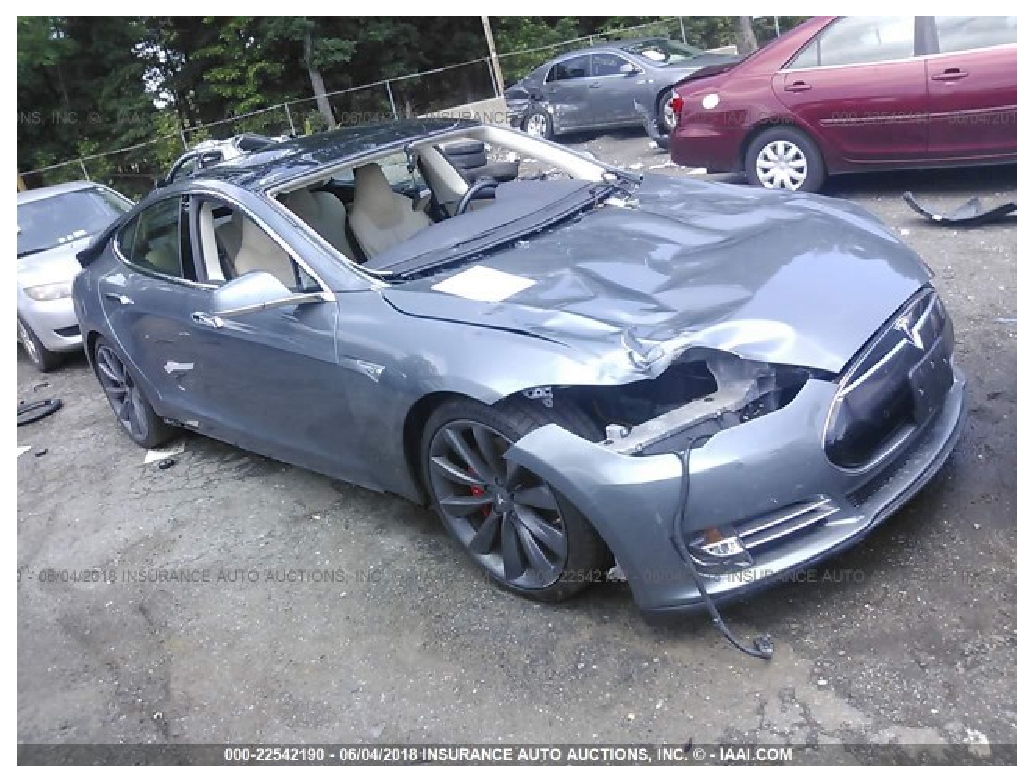
\includegraphics{model-s.eps}

\newpage
\section{Introduction}
\subsection{Purpose}
The purpose of Auction Hunter is to find the highest value car auctions for wrecked/damaged Teslas on auction website.
Our product will parse through a collection of auctions, evaluate their value, and display results to a user through a website UI. 
\subsection{Overview}
There are three primary components to our proposed product. The first part skims over car auctions using a web crawler and collects all relevant data, then saves it. The second part parses through all that saved data and performs estimations on value, which can be compared to the current asking price. The third component displays this information to the user through a website. A user will be able to search for particular characteristics to help narrow down the available auctions. They will also ultimately be the final say over which auction they choose. Images of each auction will be displayed to the user, which enables them to make a final judgment call. A stretch goal would be to use machine learning to eliminate or promote a subset of auctions based on the images provided.

\subsection{Definitions}
Web Crawler - a program that systematically collects information off of the web. This can be used to compile information or data without requiring a human to manually navigate to each web page. 

Website UI - A privately or publicly hosted website which will use an internet browser to display information to a user. It serves as a way for humans to easily interpret information that is being collected and calculated upon in the back-end. 

Wrecked Car Auctions - Insurance companies will commonly create auctions to sell cars that have crashed or been badly damaged. The insurance company will pay out an insurance holder, or replace their car. Teslas are commonly auctioned because insurance companies avoid repairing them due to high or variable repair costs. 

Highest Value Car - The cars being sold at auction have some intrinsic value. This could be the grand total of each individual part after labor has been accounted for. It could also be the total price of the car after necessary repairs have been performed. Since the cars are sold at auction, this price is more variable based on bidders' actions. An auction would be worth bidding on if the total value is greater than the current asking price. Since there are so many auctions, the best would be displayed first. 

\section{System Requirements}
A publicly hosted Auction Hunter website that displays to the user the projected value of each auction. There will also be a way for the user to sort the list of auctions to refine their search. When a user finds a high value action, they can obtain additional information such as images and a link to the original auction listing. 

This website will utilize a number of back-end scripts which crawl through wrecked car auctions (specifically Teslas) to pull all relevant data. Once the data from each auction is collected, we can predict relative values for each auction and add it to a database to be displayed to the user. 

To better judge the effectiveness of our algorithms, we can compare the value that our scripts assign to each car to the final sale price. We can also manually evaluate our predictive algorithms to verify it is assigning value correctly. We will plot any relevant performance data to present the effectiveness of our algorithms.  

%\section{System Requirements}

\subsection{User Stories}
\begin{itemize}
\item As a user, I want to be able to access Auction Hunter from anywhere.
\item As a user, I want a user interface that is easy to use.
\item As a user of Auction Hunter, I want to be able to sort a list of auctions by price, value, or model of car. 
\item As a user, I want to sort the car list by selecting price range and present or absence of VIN. 
\item To save as much money as possible, I want to make sure that I am getting a good deal on wrecked car auctions, especially for newer Teslas.
\item As a user, I want to be able to set alerts when there is a car I want up for auction
\item As a mechanic, I want to have proof that Auction Hunter is accurate in it's value predictions so I can buy parts while saving money. I also want proof that it works faster than manually evaluating auctions.
\item I want to be able to automatically bid on Auctions that match what I am looking for, in case I am away from my computer.
\item Auction Hunter should be able to scrape Auction data from IAAI and Copart.
\item Analyze auction photos to get a rough damage estimate using machine learning. 
\end{itemize}

\subsection{Functional Requirements}
At its core Auction Hunter is a website that allows users access to information it has stored in its database. The website should allow for the following functions to be preformed.

\begin{itemize}
\item User access controls to only allow signed-up users access to the Auction Hunter
\begin{itemize}
    \item Allow users to sign up to Auction Hunter
    \item Let users sign in using their email and password
    \item Reset their password if a user forgets it
\end{itemize}
\item Account page to manage user preferences
\begin{itemize}
    \item Lets user change email and password
    \item View notifications Auction Hunter has sent them about auctions
    \item Specify parameters about what types of auctions they want alerts about
\end{itemize}
\item Summary page that displays charts, graphs, averages, and pictures of auction information
\begin{itemize}
    \item Table of recent auctions order by date, with selectable criteria
    \item Each row should be simple information as well as estimated value and actual auction price
    \item Search bar to filter auctions by color, price, etc.
    \item Clicking an auction brings user to details page about it
\end{itemize}
\item Details page that display all information about a specific auction
\begin{itemize}
    \item Pictures of car
    \item Estimated value of car calculated by Auction Hunter
    \item All other data that Auction Hunter can find on auction websites
\end{itemize}
\end{itemize}

Auction Hunter also needs a way of gathering the auction data to power its website. This is done via web scraping scripts that run at automated times.

\begin{itemize}
    \item Query Copart and Iaai API's for basic auction data
    \begin{itemize}
        \item Vin
        \item Airbag and crash data
        \item Photos of vehicle and damage
        \item Options and specifics of the car
    \end{itemize}
    \item Scrape auction websites for when auctions are happening in the future
    \item Track live auctions to see final price of car
    \item Participate in auctions on behave of users
    \item Use photos of damage to try and estimate value of car (machine learning)
\end{itemize}

\subsection{Performance requirements}
Response Time: All of the response time are measured in end user environment(the browser rendering the response)
\begin{itemize}
\item Below operations must respond within 5 seconds.
\begin{itemize}
    \item “Access action hunter homepage”
    \item “Sign up”
    \item “Log in account”
    \item “Log out account”
    \item "Viewing the details of car"
    \item “Set the values of notification for coming cars”  
    \item “Set the values of automatically bid”
    \item “Sort the list of auctions by price, value, model, VIN, etc”
\end{itemize}
\item Below operations must respond within 2 minutes, and there must be a prompt message shows that the back end is still working on searching.
\begin{itemize}
    \item “Scrape Auction data from IAAI and Copart”
\end{itemize}
\item Below operations must respond within 10 minutes.
\begin{itemize}
    \item “Notice users when an auction has a car which satisfies users’ requirements”
    \item “Automatically bid on Auctions that match users’ requirements”
\end{itemize}
\end{itemize}

\begin{center}
Workload: The table below estimates that for a user scenario how many requests per day.\\
\begin{tabular}{ | m{2cm} | m{4cm}| m{3cm} | m{3cm} | } 
\hline
Ref No & Scenario & Pages & Daily Total(estimate) \\ \hline
1 &Visit homepage   &Portal  &100\\  
\hline
2 &Sort car list  &Portal  &100\\
\hline
3 &Set notification  &Login,Notification  &10\\
\hline
4 &Set automatically bid  &Login,Bid  &5\\
\hline
5 &Scrape auction data  &Portal  &80\\
\hline
6 &View notification  &Login,Notification  &10\\
\hline
7 &View bid  &Login,Bid  &5\\
\hline
8 &View car details  &Portal,CarDetails &90\\
\hline
\end{tabular}
\end{center}

\section{Testing}
To verify that the back-end algorithms assign value correctly, we will calculate the difference between the real value of the auction and the value that is assigned. We will also compare the value assigned to the final sale price of each auction to calculate the difference. We also need to make sure that the user experience is intuitive.

\subsection{User Testing}
As a stretch goal, we could get some users unaffiliated with this project to try out our final website to provide feedback. 

\subsection{Continuous Integration}
During the development of Auction Hunter we will integrate our code repository with a build system to automatically run regression and unit tests every time we make a change to the master branch. The unit tests will be written by the owner of each sub-component of the website and backend script. The regression tests will need to be maintained by the whole group as we continue to expand the project. This will allow us to catch simple bugs quickly and efficiently in order to prevent bad code from making its way into our code base overtime. 

\section{Schedule}
\begin{ganttchart}[hgrid,vgrid]{1}{28}
    %Fall
    \gantttitle{2018-2019 By Week (Ignoring Breaks)}{28} \\
    \gantttitlelist{1,...,28}{1} \\
    \ganttgroup{Fall 2018}{1}{6} \\
    \ganttgroup{Winter 2019}{7}{17} \\
    \ganttgroup{Spring 2019}{18}{28} \\
    \ganttbar{Requirements Draft}{1}{2} \\
    \ganttlinkedbar{Requirements Final}{3}{5} \\
    \ganttbar{Tech Review Draft}{1}{2} \\
    \ganttbar{Design Document}{4}{6} \\
    \ganttlinkedbar{Client Verification}{5}{6} \\
    \ganttbar{Info Interview}{5}{6} \\
    
    %Winter
    \ganttbar{Basic Web Crawling}{7}{9}\\
    \ganttlinkedbar{Backend Database}{8}{10}\\
    \ganttlinkedbar{Website }{10}{13}\\
    \ganttlinkedbar{Value Calc}{8}{12}\\
    \ganttlinkedbar{Incorporate Components}{13}{17}\\
    
    
    %Spring
    \ganttbar{Finalize Implementation}{18}{20}\\
    \ganttlinkedbar{Verification}{20}{22}\\
    \ganttlinkedbar{Real world testing}{22}{24}\\
    \ganttlinkedbar{Prepare for expo}{24}{28}\\
    
    %\ganttlinkedbar{Task 2}{3}{7} \ganttnewline
    \ganttmilestone{Expo}{28} \ganttnewline
\end{ganttchart}

\end{document}
